\documentclass[12pt,oneside]{article}
\usepackage{enumerate}
\usepackage{fancyhdr}
\usepackage{a4wide}
\usepackage{titlesec}
\usepackage{enumitem}
\usepackage[utf8]{inputenc}
\usepackage{graphicx} % Required for inserting images
\usepackage{tocloft}
\usepackage[table]{xcolor}
\usepackage{ragged2e}

\setlength{\arrayrulewidth}{0.5mm}
\setlength{\tabcolsep}{10pt}
\renewcommand{\arraystretch}{2.5}

\usepackage{longtable}
\definecolor{lightblue}{HTML}{b0c4de}
\definecolor{lightsteelblue}{HTML}{add8e6}

\usepackage{hyperref}

\usepackage{floatrow} 
\usepackage{graphicx}
\usepackage[export]{adjustbox}
\usepackage{wrapfig}
\usepackage{subcaption}

\usepackage[absolute,overlay]{textpos}

%%%%%%%%%%%%%%%%%%%%%%%%%%%%%%%%
\begin{document}

%pagina introduttiva
\begin{titlepage}
    \begin{flushright}
        \textbf{Corso di Fondamenti di Intelligenza Artificiale}
        \textbf{\\Università degli Studi di Salerno}
    \end{flushright}
    \vspace*{1.5cm}
    \centering
    \includegraphics[width=0.4\textwidth]{pics/logoUNISA.png}
    \vfill
    \Huge\textbf{BOOK CATEGORIZATION}
    \vspace{1ex}
    \rule{\linewidth}{1pt}
    \Large\textbf{Mancuso Maria Angela \\
        Malfettone Ines \\
        Santonicola Federico  \\
        Sessa Attilio \\
        }
    \rule{\linewidth}{1pt}
    \vspace{2cm}
    \hfill
    \textit{\href{https://github.com/fedesanto/ProgettoFIA}{Link GitHub}}
    \hfill
    \vfill
    \today
\end{titlepage}

%indice
\clearpage %crea nuova pagina

\setcounter{page}{1}

\begin{flushright}
        \Large\textbf{Indice}
\end{flushright}
\rule{\linewidth}{1pt}

\renewcommand{\contentsname}{}
\tableofcontents

%1
\clearpage
\setcounter{section}{0}
\section{Introduzione}
    \begin{enumerate}
    \subsection{Scopo del progetto}
    \begin{justify}

        Il nostro progetto si pone come obiettivo lo studio e la sperimentazione di differenti tecniche di Machine Learning capaci di analizzare ed estrarre informazioni da dati sotto forma di linguaggio naturale. Nello specifico si è interessati alla categorizzazione di libri tramite una breve descrizione testuale ed un elenco di autori. La categorizzazione è stata elaborata tramite due tecniche di Machine Learning: Classificazione e Clustering, che, seppur facenti utilizzo di due approcci diversi (rispettivamente apprendimento supervisionato e apprendimento non supervisionato), si considerano in grado di riportare risultati similari e confrontabili. A tal proposito occorrerà addestrare più modelli differenti riguardanti entrambe le tecniche e verificare quali di questi permetterà di ottenere il miglior risultato.

    \end{justify}
    \end{enumerate}

\hfill
\hfill
\section{Specifiche del progetto}
    \begin{enumerate}
        \subsection{Ambiente: PEAS}
   
%tabella
    \centering
    \begin{longtable}{ | p{3cm} | p{11cm} | }\hline
    \multicolumn{2}{|c|}{PEAS} \\ \hline
    \rowcolor{lightblue}
    \textbf{Performance} & La misura di prestazione è la capacità di avvicinarsi quanto più possibile al corretto genere di un libro specifico. È necessario utilizzare misure di prestazione differenti con lo scopo di valutare gli algoritmi di Classificazione e Clustering. Nel caso della Classificazione si è usato: accuratezza e report di classificazione. Quest'ultimo comprende la misura di precisione, recall, f1-score (per ciascuna classe) e una matrice di  confusione tramite la quale è possibile visualizzare l'andamento degli algoritmi. Per il clustering, invece,  si è utilizzato il Silhouette Score.\\
    \hline
    \rowcolor{lightsteelblue}
    \textbf{Environment} & I modelli presi in considerazione sono stati realizzati e operano nell'ambiente di sviluppo "PyCharm" avente le seguenti caratteristiche: \begin{itemize}
        \item \textbf{completamente osservabile}: il modello ha la visione completa del dataset, nello specifico degli attributi associati a ciascun libro.
        \item \textbf{deterministico}: una volta addestrato un modello, lo stato dell'ambiente non varia a fronte degli stessi input.
        \item \textbf{episodico}: l'agente delibera a fronte di determinati episodi che consistono in nuove richieste di predizione.
        \item \textbf{statico}: l'ambiente resta invariato mentre l'agente opera.
        \item \textbf{discreto}: è fornito un insieme discreto di informazioni per ciascun libro.
        \item \textbf{singolo}: l'ambiente permette di addestrare più modelli valutati singolarmente.
    \end{itemize}
    \hline
    \rowcolor{lightblue}
    \textbf{Actuators} & Gli agenti mostrano i risultati attraverso due tipi di attuatori: \begin{itemize}
    \item console dell'ambiente di sviluppo: durante l'addestramento e testing i modelli riportano informazioni di controllo e i risultati ottenuti.
    \item grafici esplicativi: mostrano informazioni di vario tipo, tra cui analisi del dataset e risultati ottenuti dalle predizioni dei modelli.\end{itemize}
    \hline
    \rowcolor{lightsteelblue}
    \textbf{Sensors} & I modelli ricevono le informazioni necessarie per l'addestramento tramite un file in formato csv contenente il dataset. Inoltre, è possibile specificare, grazie all'utilizzo della console, nuovi dati su cui effetturare nuove predizioni. \\
    \hline
    \caption{Tabella della specifica PEAS}
    \end{longtable}
\label{table:ta}
\end{enumerate}

\begin{enumerate}
\subsection{Metodologie utilizzate}\label{due}
    \begin{justify}
        Come si evidenzia dallo scopo del progetto, ci si trova ad affrontare un’istanza di un problema di analisi testuale in linguaggio naturale. Tale classe di problemi risulta così complessa, ma anche così rilevante nell’ambito del machine learning, da essersi meritata una disciplina a sé nota come NLP (Natural Language Process). In genere, analizzare un testo in linguaggio naturale è molto complesso per differenti motivi, tra cui:
        \begin{itemize}
            \item Ambiguità del linguaggio;
            \item Uno stesso concetto può essere espresso in molti modi differenti;
            \item Errori di ortografia;
            \item Parole “rumorose” che non aggiungono significato;
        \end{itemize}
        Tuttavia, nel nostro contesto non è necessario concentrarsi sull’estrazione di semantica, in un testo in cui la semantica è nascosta, ma è molto più importante evidenziare la presenza di parole chiave che ci permettano di determinare la categoria di appartenenza di un dato libro. 
        A titolo di esempio, si prenda in considerazione la seguente descrizione: 
        \textit{“Dei cavalieri affrontano ed uccidono un drago in un regno lontano”}.
        Ai fini del nostro scopo non è importante dedurre informazioni contestuali o semantiche (come il fatto che avvenga uno scontro) ma è sufficiente notare la presenza di determinate parole (come “\textit{cavalieri}”, “\textit{drago}”, “\textit{regno}”) per dedurre la categoria del libro (in questo caso “\textit{Fantasy}”).
        Notato ciò, la nostra attenzione si pone su una specifica tecnica di NLP detta “Bag of Words”, il cui funzionamento consiste nella creazione di un vocabolario di tutte le differenti parole presenti in un corpus di testi e ciascuno documento sarà rappresentato da un vettore di conteggi delle parole presenti. È evidente che, se una determinata descrizione contiene un gran numero di parole come “\textit{cucina}” o “\textit{ricetta}”, è molto più probabile che si tratti di un libro di cucina, piuttosto che un romanzo.
        Nonostante ciò, risulta comunque opportuno effettuare delle operazioni di pulizia del testo che ci permettano di ridurre il “rumore” e rendere descrizioni e autori più uniformi. Ad esempio, sono moltissime le parole che non danno nessun tipo di contributo alla determinazione della categoria (come tutte le congiunzioni o parole ridondanti come “\textit{book}” o “\textit{new}”) la cui rimozione permetterebbe di evidenziare maggiormente termini più significativi (si veda il paragrafo \ref{tre}).

    \end{justify}
\end{enumerate}

\newpage
\section{Analisi e preparazione dei dati}
    \begin{enumerate}
    \subsection{Scelta del dataset}
    \begin{justify}
    Per lo scopo di tale progetto si è scelto un dataset già esistente, reperibile \href{https://www.kaggle.com/datasets/elvinrustam/books-dataset}{qui}. La ricerca del dataset si è basata sulla necessità di trovarne uno contenente libri provveduti di descrizione e autori. Il dataset scelto fornisce informazioni relative a 103063 libri ed ha una dimensione di 69.75MB. Tutti i dati sono in formato testuale.
    \end{justify}
    \end{enumerate}

    \begin{enumerate}
    \subsection{Data cleaning}\label{tre}
    \begin{justify}
    Nella fase di Data Cleaning ci si occupa di "pulire" il dataset mantenendo solo i dati utili all'addestramento del modello. Da una prima osservazione dei dati è stata rilevata la presenza di due aspetti che possono ostacolare la corretta esecuzione degli algoritmi di classificazione e di clustering, che saranno implementati successivamente. La funzione "clearData" si occupa della pulizia dei dati, con le seguenti operazioni: 
    \begin{enumerate}[label=\arabic*)]
        \item eliminazione dei campi nulli. In tal modo si è ottenuto un dataset senza dati mancanti.
        \item eliminazione delle righe duplicate.
        \item eliminazione delle righe non significative. Per identificare le frasi non significative è stato utilizzato il parametro "des\textunderscore{}threshold" che indica un limite. Se le frasi contengono un numero di caratteri inferiore a "des\textunderscore{}treshold" allora verranno considerate non significative.
    \end{enumerate}
    La funzione "clearData" applica la prima e la seconda operazione su tutti i dati presenti all'interno del dataset. Mentre la terza operazione verrà eseguita solo sulla feature delle descrizioni, in quanto applicarla agli autori potrebbe risultare controproducente. 
    \end{justify}
    \includegraphics[width=0.95\textwidth]{pics/cleanData.png}
    
    \newpage
    \begin{justify}
    Dopo una successiva analisi del dataset e delle categorie presenti al suo interno, si è notata la presenza di alcune categorie similari. Per assicurarci una predizione ottimale del genere è necessario identificare le categorie nella loro unicità. A tale scopo viene utilizzata la funzione "renameCategories". Essa si occupa di rinominare le categorie utilizzando una lista di rinominazioni.
    \end{justify}

    \includegraphics[width=0.95\textwidth]{pics/renameCategories.png}

    \begin{minipage}[t]{0.39\textwidth}
    \vspace{30pt}
    Di lato è mostrata la lista passata alla funzione "renameCategories":
    \end{minipage}
    \hfill
    \begin{minipage}[t]{0.50\textwidth}
    \vspace{20pt}
    \includegraphics[width=1\textwidth]{pics/rinominoCategorie.png}
    \end{minipage}
    
    \begin{justify}
    Sono state selezionate sedici categorie differenti. Tale selezione è stata effettuata prendendo in considerazione la frequenza della ricorrenza di ciascuna categoria. Questo ha portato all' eliminazione di categorie aventi troppi pochi dati per permettere ai modelli di ottenere un buon riconoscimento della categoria stessa. Tale operazione viene effettuata tramite la funzione "extractCategories".
    \end{justify}

    \begin{justify}
    La seguente funzione si occupa di estrarre le categorie di interesse in modo da poter eliminare tutte quelle righe non appartenenti ad esse. 
    Per ogni riga vengono svolte le seguenti azioni:
    \begin{itemize}
        \item estrarre tutte le categorie separate da ',';
        \item se nessuna delle categorie estratte appartiene a 'toExtract', allora la riga viene eliminata;
        \item tra le categorie che fanno parte di 'toExtact', viene assegnato al campo "Category" quella che ha meno esempi nel dataframe.
    \end{itemize}
    \end{justify}

    \includegraphics[width=0.95\textwidth]{pics/extractCategories.png}

    \begin{justify}
    Di seguito sono mostrate le categorie estratte: 
    \end{justify}
    \includegraphics[width=0.95\textwidth]{pics/listaCategories.png}

    \begin{justify}
    Lavorare su dati testuali significa lavorare sul Natural Language. Quest'aspetto implica una sequenza di azioni di normalizzazione da applicare sulle descrizioni e sugli autori. Ma prima di normalizzare i dati risulta più efficiente eseguire un'operazione di bilanciamento del dataset (vedere paragrafo ~\ref{bil}) nel quale vengono eliminate le righe di quelle categorie troppo frequenti.
    Le operazioni di normalizzazione sono svolte dalle funzioni "preprocessAuthors" e "preprocessDescription". Queste funzioni utizzano le stop words che vengono identificate prima della loro esecuzione. Tramite l'utilizzo delle librerie NLTK sono state individuate le stop words e sono state successivamente aggiunte ai file "authors\textunderscore{}stopwords.txt" e "description\textunderscore{}stopwords.txt" in modo da distinguere le stop words all'interno delle features "authors" e "descriptions". 
    \end{justify}
    \newpage
    \hfill
    \hfill
    \begin{justify}
    \hypertarget{preD}{
    La funzione "preprocessDescrition" esegue le seguenti operazioni:
    \begin{itemize}
        \item i caratteri vengono resi tutti minuscoli in modo da rendere i dati testuali più uniformi e leggibili;
        \item eliminazione della punteggiatura per eliminare il rumore;
        \item eliminazione delle stop words;
        \item lemmatizzazione, una tecnica che permette la riduzione delle parole nella loro forma radice considerando sia la grammatica che il significato (esempio: \textit{playing play}).
    \end{itemize}
    }
    \end{justify}
    
    \hfill
    \hfill
    
    \includegraphics[width=0.95\textwidth]{pics/preprocessDescription.png}
    \newpage
    \begin{justify}
    \hypertarget{preA}{
    La funzione "preprocessAuthors" eseguirà le stesse prime tre operazioni di "preprocessDescription".
    }
    \end{justify}
    
    \includegraphics[width=0.95\textwidth]{pics/preprocessAuthors.png}
    \begin{justify}
    Per illustrare la corretta esecuzione delle due funzioni mostrate precedentemente vengono utilizzate le WordCloud (vedere capitolo \ref{word}). Queste vengono utilizzate per osservare facilmente come i dati testuali siano cambiati e resi più semplci e funzionali.
    In conclusione, dopo la fase di Data Cleaning, avremmo un database completo e leggibile che garantisca sia la qualità che la quantità dei dati. 
    \end{justify}
    \end{enumerate}
    

    \begin{enumerate}
    \subsection{Feature Selection}
    \begin{justify}
    Il dataset orginale presentava sette features diverse: Title, Authors, Description, Category, Publisher, Publish Date e Price. Per lo scopo del nostro progetto verrano prese in considerazioni solo le feature che contengono: il titolo, per una questione di chiarezza, la descrizione e gli autori, poiché sono le due caratteristiche che utilizzeremo per predirre il genere del libro, e il genere per organizzare i libri e valutare se la predizione ha dato esito positivo.
    \end{justify}
    \end{enumerate}

    \newpage
    \begin{enumerate}
    \subsection{Bilanciamento dataset}\label{bil}
    \begin{justify}
    %sistema l'ordine
    Da una prima osservazione del grafico, che mostra i libri divisi nei 20 generi, si può notare lo sbilanciamento del dataset. 
    \end{justify}
    
    \begin{figure}[H]
    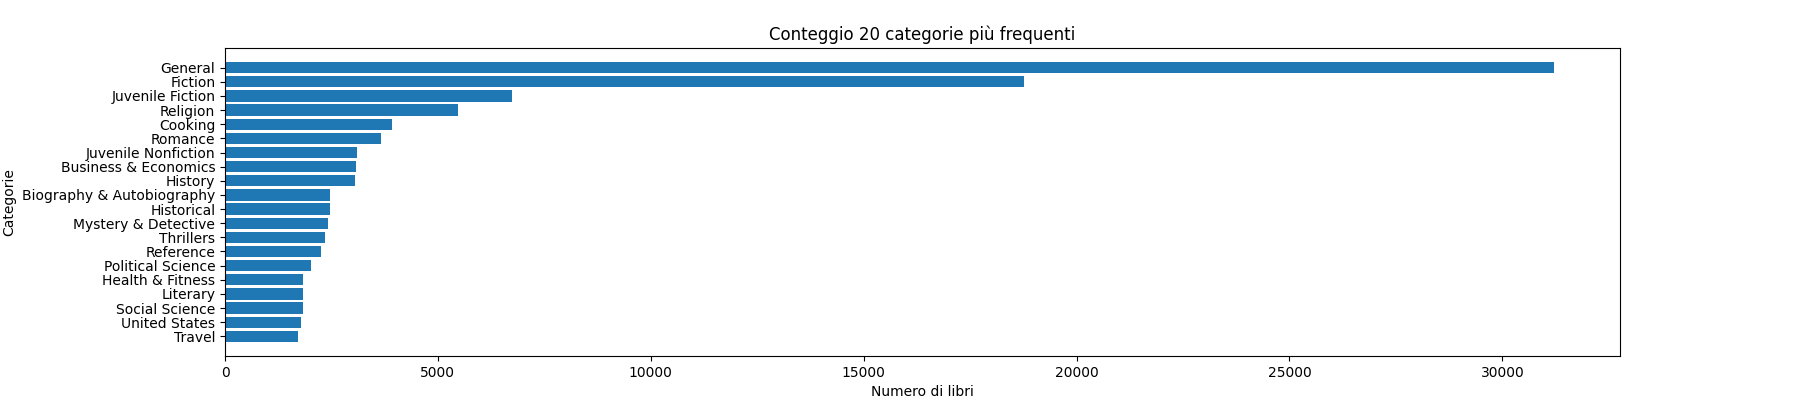
\includegraphics[width=1\textwidth]{pics/dati_iniziali.png}
    \caption{Database non bilanciato}
    \end{figure}

    \hfill
    \begin{justify}
    Dunque, per ovviare a problemi di overfitting, si è ritenuto necessario bilanciarlo quanto più possibile. Si passa dunque al seguente dataset:
    \end{justify}
    
    \begin{figure}[H]
    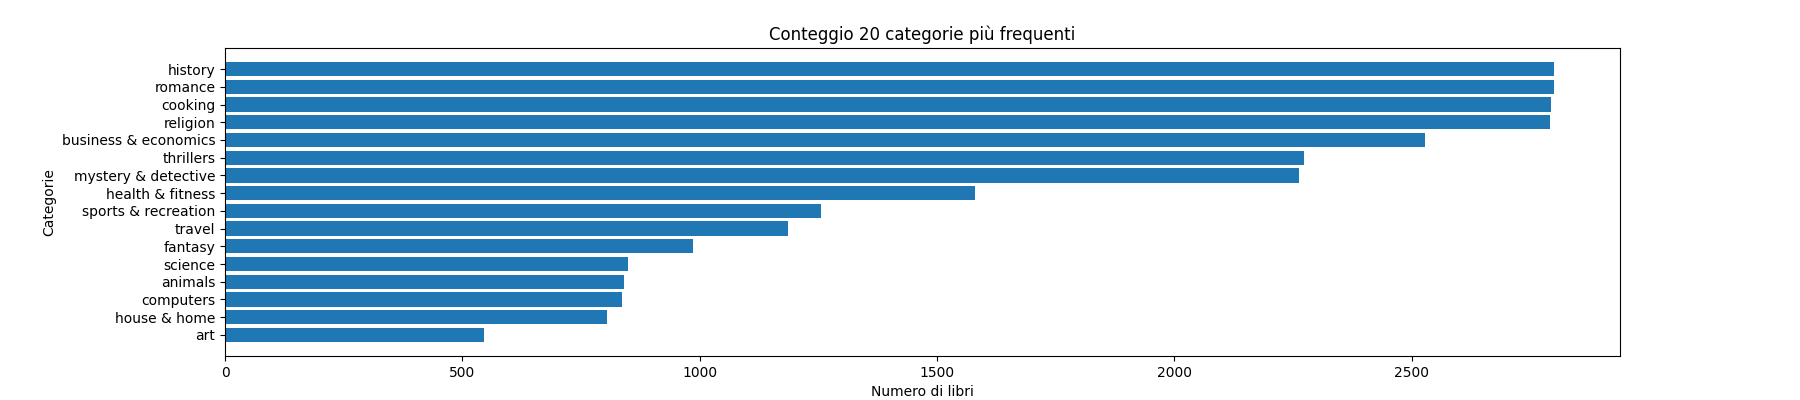
\includegraphics[width=1\textwidth]{pics/dati_postprocessati.png}
    \caption{Database bilanciato}
    \end{figure}
    
    \begin{justify}
    Come si nota dalla 'Figure 2' il dataset non risulta completamente bilanciato. Questo risultato è dovuto alla natura stessa del dataset. Per ottenere un dataset bilanciato si sarebbero dovute eliminare molte informazioni, non avendo così più a disposizione abbastanza dati per addestrare i nostri modelli.\\
    \end{justify}

    \newpage
    \begin{justify}
    Il bilanciamento del dataset è stato effettuato tramite la funzione "balanceCategories", la quale verifica il numero di righe per ogni categoria ed elimina casualmente delle righe di categorie con più di 'threshold' esempi.
    \end{justify}
    \includegraphics[width=0.95\textwidth]{pics/balanceCategories.png}
    

    \begin{minipage}[t]{0.40\textwidth}
    \vspace{30pt}
    Possiamo concludere che sono state effettuate le seguenti modifiche del dataset in questione, con la rimozione del seguente numero di righe:
    \end{minipage}
    \hfill
    \begin{minipage}[t]{0.50\textwidth}
    \vspace{20pt}
    \includegraphics[width=1\textwidth]{pics/bilanciamento.png}
    \end{minipage}
    \end{enumerate}


    \hfill
    \begin{enumerate}
    \subsection{Visualizzazione Word Cloud}\label{word}
    \begin{justify}
    Word Cloud è una tecnica per la visualizzazione dei dati. È utilizzata per rappresentare dati di testo in cui la dimensione di ciascuna parola ne indica l'importanza.\\
    Grazie all'utilizzo delle WordCloud, nello specifico tramite l'utilizzo delle funzioni "createDescriptionWordCloud" e "createAuthorsWordCloud", è stato possibile illustrare le parole chiavi presenti all'interno delle descrizioni e degli autori. Verrano creati tanti WordCloud quante sono le categorie.
    \end{justify}
    \includegraphics[width=0.95\textwidth]{pics/descriptionWordCloud.png}

    \begin{justify}
    La seguente immagine è un esempio di output della funzione (con lo scopo di farne comprendere il corretto funzionamento, vengono mostrate solo quattro categorie):
    \end{justify}
    \begin{figure}[H]
    \centering
    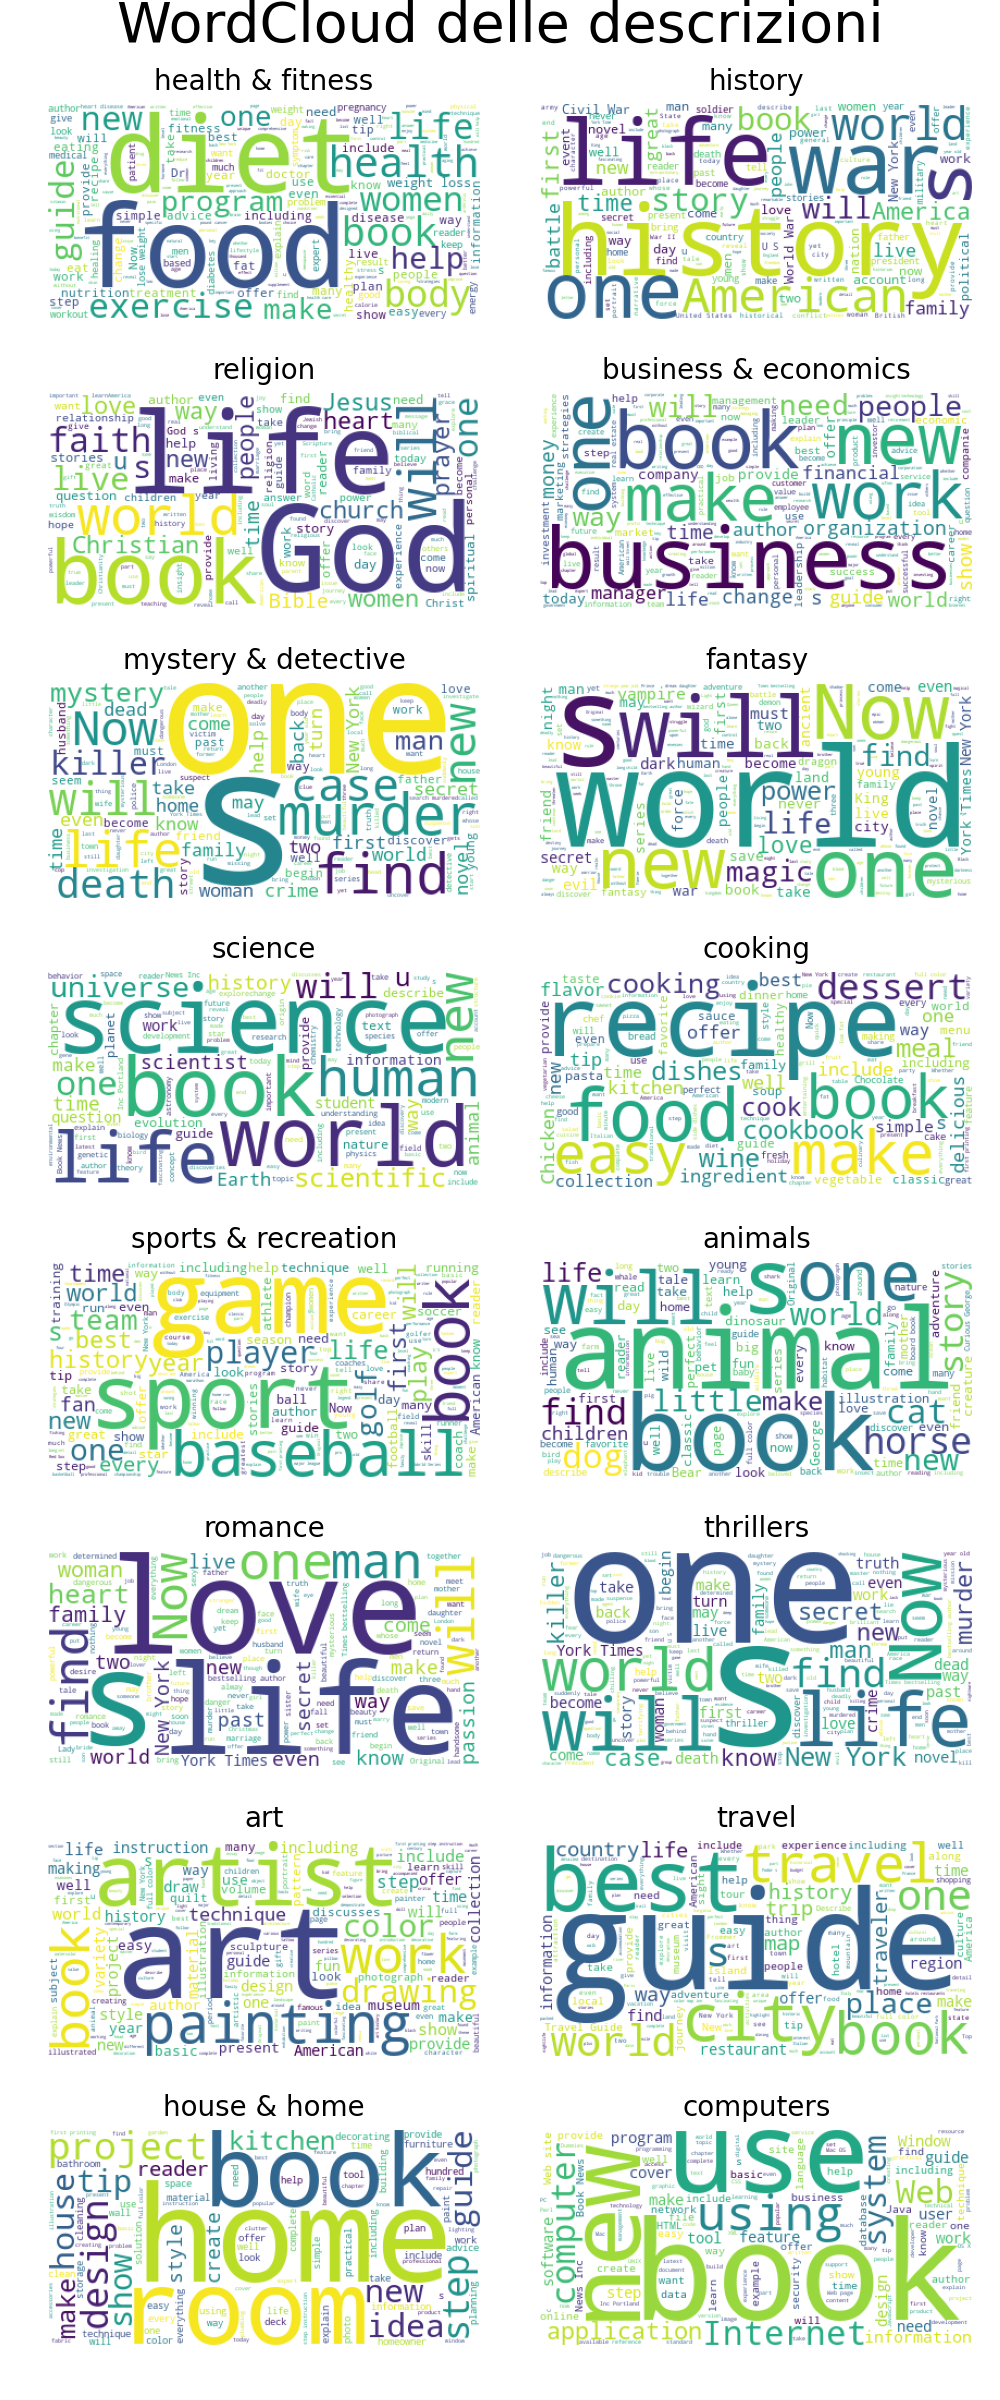
\includegraphics[width=0.90\textwidth]{pics/wordcloud_descrizioni_nonprocessate.png}
    \caption{Word Cloud delle descrizioni non processate}
    \end{figure}


    \begin{justify}
    Tale illustrazione ci permette di analizzare con più semplicità le parole ricorrenti ed individuare delle stop words aggiuntive, che fanno riferimento al dataset in questione, come ad esempio "\textit{book}" e "\textit{life}". Allo stesso ragionamento vengono sottoposti gli autori. Per le stop words aggiuntive, inerenti alla descrizione e agli autori, sono stati creati due nuovi file di testo, chiamati rispettivamente "description\textunderscore{}stopwords.txt" e "authors\textunderscore{}stopwords.txt". Di seguito sono mostrate le stop word individuate:
    \end{justify}
    
    \begin{figure}[H]
    \begin{subfigure}{0.10\textwidth}
    \includegraphics[width=\linewidth]{pics/aggiuntaStopWordsDescription.png} 
    \begin{justify}
    \caption{Stop Word delle descrizioni}  
    \end{justify}
    \label{fig:subim1}
    \end{subfigure}
    \hspace{3cm}
    \begin{subfigure}{0.11\textwidth}
    \includegraphics[width=\linewidth]{pics/aggiuntaStopWordsAutori.png}
    \begin{justify}
    \caption{Stop Word degli autori}   
    \end{justify}
    \label{fig:subim2}
    \end{subfigure}
    \caption{Stop Word aggiunte}
    \end{figure}

    \newpage
    \begin{justify}
    L'eliminazione delle stop words avviene tramite le funzioni \hyperlink{preD}{"preprocessDescription"}, per le descrizioni, e \hyperlink{preA}{"preprocessAuthors"}, per gli autori. Si ottiene il seguente word cloud riguardanti le descrizioni:
    \end{justify}
    \begin{figure}[H]
    \centering
    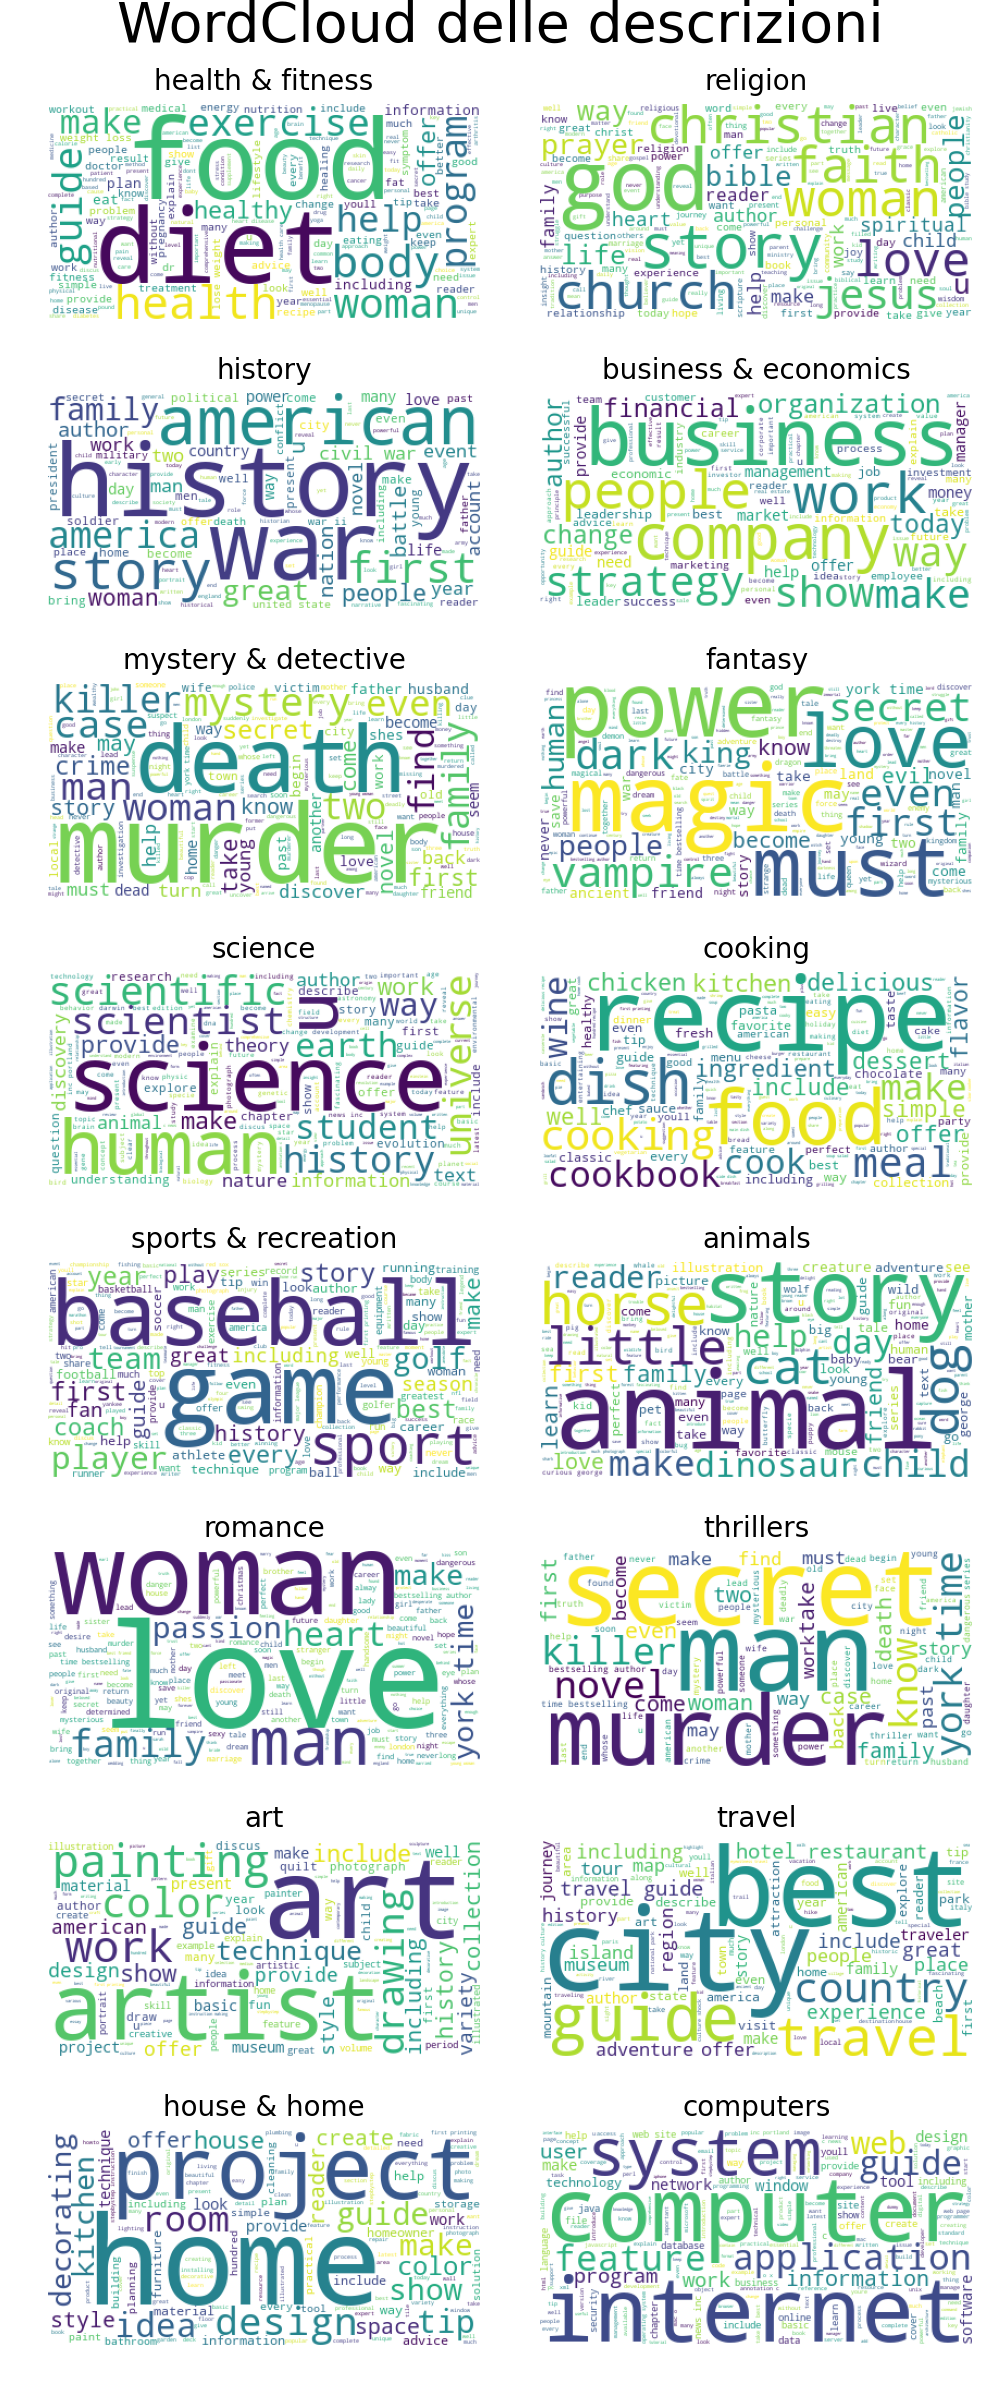
\includegraphics[width=0.95\textwidth]{pics/wordcloud_descrizioni_processate.png}
    \caption{Word Cloud delle descrizioni processate}
    \end{figure}

    \hfill
    \hfill
    \begin{figure}[H]
    \begin{subfigure}{0.48\textwidth}
    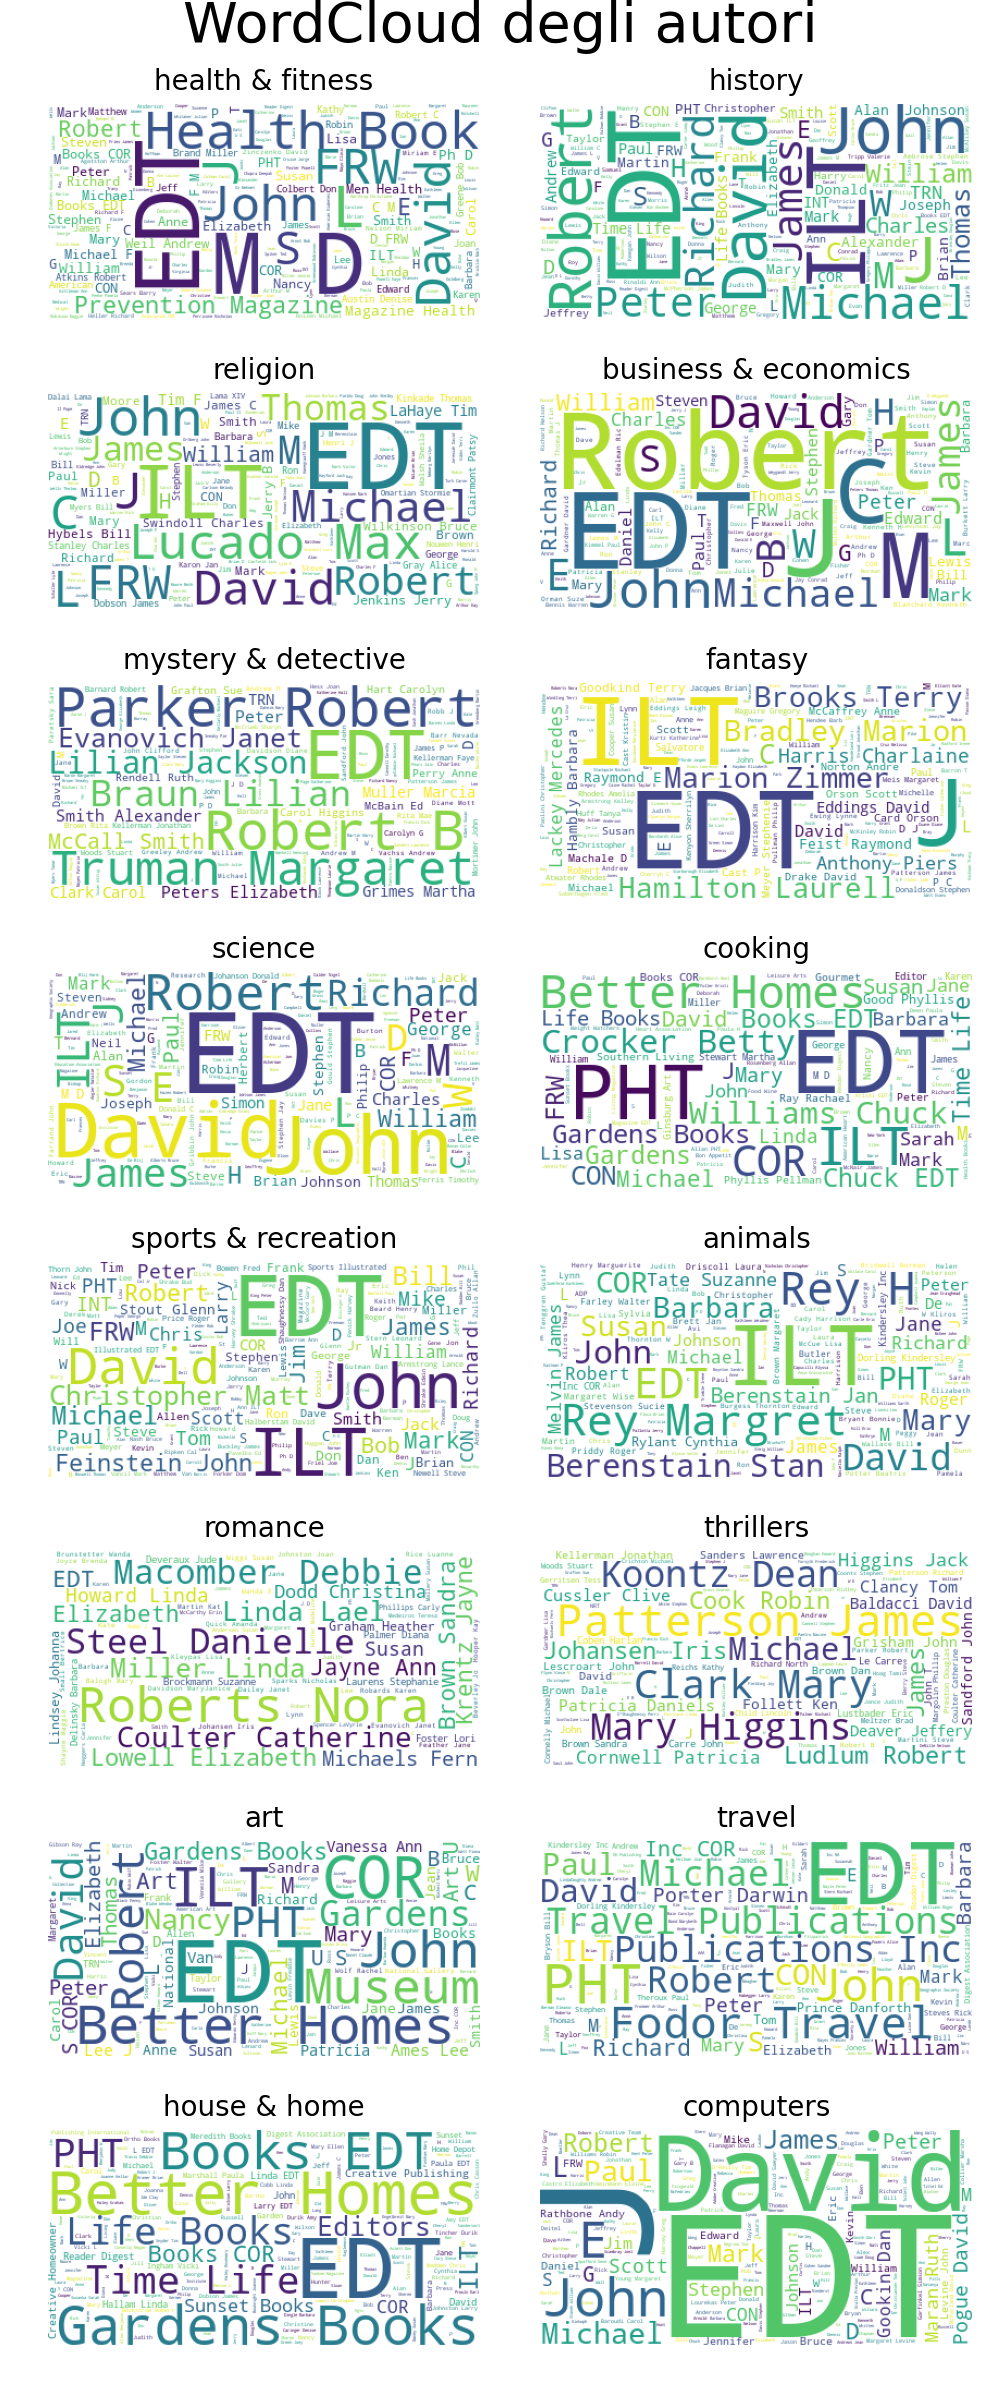
\includegraphics[width=\linewidth]{pics/wordcloud_autori_nonprocessati.png} 
    \caption{Word Cloud degli autori non processati}
    \label{fig:subim1}
    \end{subfigure}
    \begin{subfigure}{0.48\textwidth}
    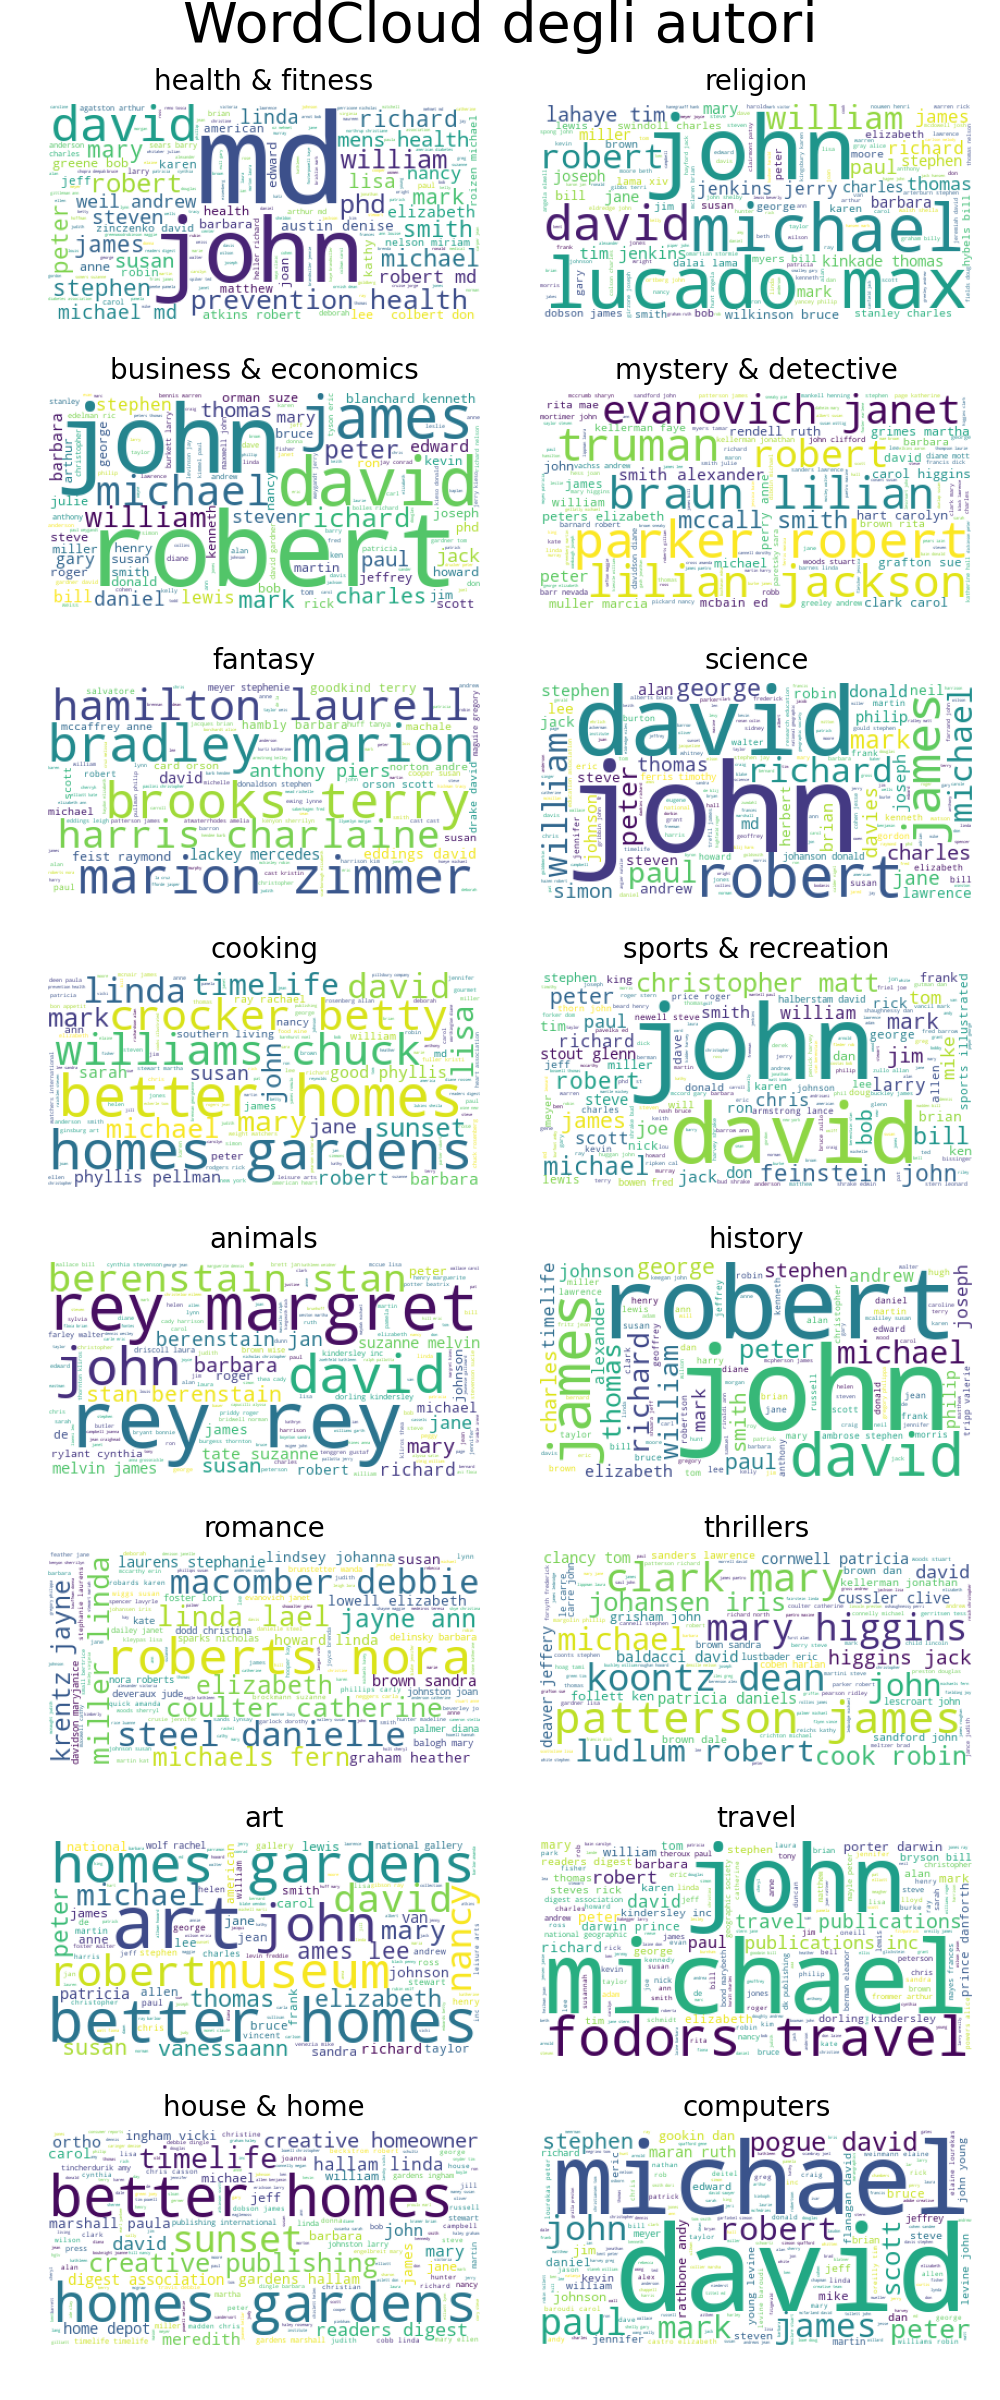
\includegraphics[width=\linewidth]{pics/wordcloud_autori_processati.png}
    \caption{Word Cloud degli autori processati}
    \label{fig:subim2}
    \end{subfigure}
    \caption{Word Cloud degli autori}
    \end{figure}
    \end{enumerate}



    \begin{enumerate}
    \subsection{Formattazione dei dati}
    \begin{justify}
    Dopo le opportune operazioni di preparazione del dataset, è necessario rendere i dati testuali utilizzabili dai modelli di machine learning. Com’è già stato specificato precedentemente (si veda paragrafo ~\ref{due}), il testo verrà convertito in vettori di numeri, rappresentanti i conteggi delle singole parole. 
    Affinché l’addestramento dei modelli avvenga adeguatamente, è necessario effettuare un’operazione di normalizzazione di tali conteggi. In questo modo si garantisce che testi riguardanti la stessa categoria, ma con un numero di parole chiave differenti, abbiano uno stesso peso in fase di addestramento (altrimenti si rischierebbe di sovrastimare testi lunghi e sottostimare testi corti). 
    La tecnica di normalizzazione tipicamente utilizzata sui conteggi di “Bag of words” è detta TF-IDF (term frequency–inverse document frequency) la quale consente di riportare i conteggi sotto forma di frequenze, soppesate per un contributo direttamente proporzionale al numero di volte che la parola è contenuta nel documento e inversamente proporzionale al numero di documenti in cui questa è presente. Dunque viene data maggior importanza a parole molto frequenti in un documento ma abbastanza uniche e significative da non essere presenti in tanti documenti differenti.

    \end{justify}
    \end{enumerate}


\section{Classificazione}
    \begin{justify}
        La classificazione fa uso di tecniche di apprendimento supervisionato al fine di predire la variabile target (Category) sulla base delle variabili indipendenti (Descriptions, Authors).
        Esistono svariati modelli di classificazione che operano sotto condizioni ed ipotesi differenti: alcuni di questi sono più adatti per dataset sbilanciati, altri per lavorare con matrici sparse (come quella ottenuta dall’elaborazione dei testi tramite TF-IDF), ecc. Nel nostro contesto, la classificazione basata su linguaggio naturale presenta molte problematiche per le quali non è possibile identificare un modello adatto alla loro risoluzione. A tal proposito, differenti modelli di classificazione sono stati addestrati e valutati, avendo cura di garantire un confronto equo con l'utilizzo degli stessi dati in tutti i modelli sia per l’addestramento che per il testing.
        Per ogni modello sono state calcolate e riportate le seguenti metriche:
        \begin{itemize}
            \item Accuracy;
            \item Tempo necessario per l’addestramento;
            \item Classification report: precisione, recall e f1-score per ciascuna classe predetta;
            \item Matrice di confusione delle predizioni effettuate.
        \end{itemize}
    \end{justify}

   \newpage
    \begin{enumerate}
    \subsection{Mulinomial Naive Bayes Classification}
    \begin{justify}
        Il classificatore Multinomial Naive Bayes è una tipologia di classificatore probabilistico bayesiano che lavora secondo l’assunzione per cui le caratteristiche predittive siano organizzate secondo una distribuzione multinomiale. Risulta particolarmente adatto nei contesti in cui le caratteristiche degli elementi da predire rappresentano conteggi di occorrenze. Tuttavia, nel pratico anche i conteggi frazionari dovrebbero funzionare sufficientemente bene.
        Il suo addestramento ha impiegato all’incirca 5.14 secondi, ottenendo un punteggio di accuracy di 0.715. 
        Di seguito ne si riporta il suo classification report e la matrice di confusione delle predizioni:
    \end{justify}
    \centering
    \includegraphics[width=0.80\textwidth]
    {pics/classificationReport_MultinomialNB.png} 
    
    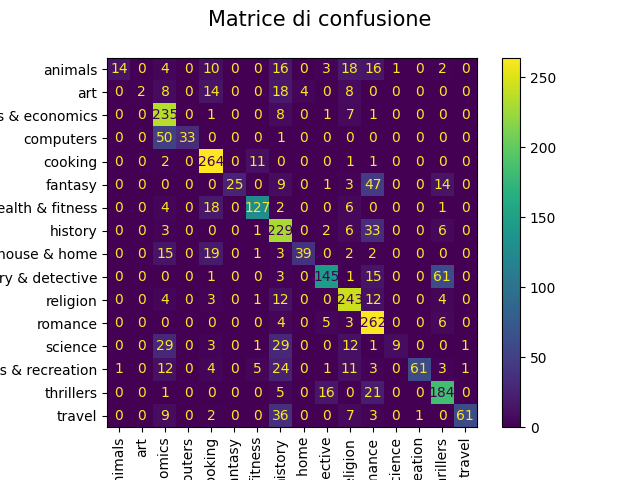
\includegraphics[width=0.95\textwidth]{pics/MultinomialNB_confusion_matrix.png}

    \begin{justify}
        Tra tutti i classificatori provati, questo è risultato essere quello più rapido durante l’apprendimento, a discapito di un punteggio di accuracy e, in generale, di risultati nettamente inferiori rispetto agli altri. Si può notare, infatti, come il modello faccia confusione su diverse categorie, non riuscendo a distinguerle da altre (si notino le predizioni fatte per “\textit{Animals}” e “\textit{Art}”). Le categorie su cui presenta più difficoltà sono di fatto quelle con minor numero di esempi all’interno del dataset, rispecchiando quelle che sono le problematiche principali di un qualsiasi classificatore bayesiano.
    \end{justify}
    \end{enumerate}

    \newpage
    \begin{enumerate}
    \subsection{Complement Naive Bayes Classification}
    \begin{justify}
        Il classificatore Complement Naive Bayes è una variante del classificatore bayesiano multinomiale, progettato per affrontare situazioni in cui le classi del problema in esame risultino particolarmente sbilanciate. Nonostante i risultati mediocri riportati dal precedente classificatore, si è comunque deciso di provate un ulteriore classificatore bayesiano per verificare se l’approccio adottato dal Complement risulti maggiormente adatto a dataset sbilanciati rispetto al Multinomial.
        Il suo addestramento ha impiegato all’incirca 5.75 secondi, ottenendo un punteggio di accuracy di 0.818. 
        Di seguito ne si riporta il suo classification report e la matrice di confusione delle predizioni:
    \end{justify}

    \centering
    \includegraphics[width=0.80\textwidth]{pics/classificationReport_ComplementNB.png}
    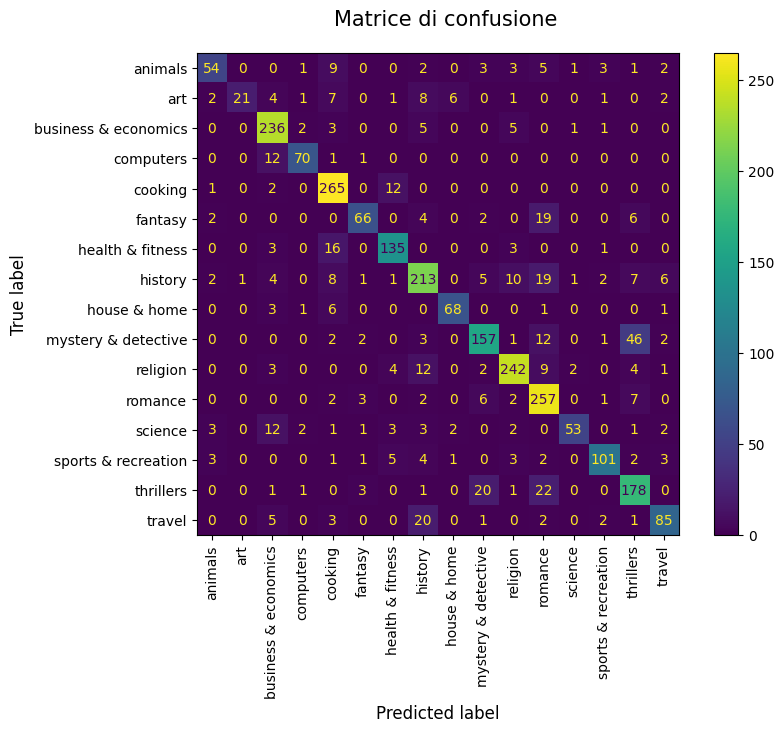
\includegraphics[width=0.95\textwidth]{pics/ComplementNB_confusion_matrix.png}

    \begin{justify}
    È possibile notare, fin da subito, risultati nettamente migliori rispetto al classificatore multinomiale, con un tempo di addestramento che, seppur leggermente superiore, è comunque paragonabile al precedente. Osservando la matrice di confusione, come ci si può aspettare da un classificatore bayesiano, si osservano ancora delle lacune nelle predizioni delle classi aventi meno esempi. Nonostante ciò, risulta evidente che l’approccio adottato dal classificatore Complement, per dataset sbilanciati, ha permesso al modello di adattarsi meglio ai dati disponibili e, seppur non ottimo per un problema di classificazione di testi, è comunque un modello valido e consigliabile in altri contesti.
    \end{justify}
    \end{enumerate}

    \newpage
    \begin{enumerate}
    \subsection{Liner Support Vector Classification}
    \begin{justify}
        Il classificatore Linear Support Vector è una tipologia di classificatore lineare binario. Il suo funzionamento è basato sulla rappresentazione degli esempi da predire, come punti in uno spazio multidimensionale, ed ha l’obiettivo di identificare il piano che meglio separa tali esempi in due categorie ben distinte. Essendo un classificatore binario, normalmente è in grado di classificare solo due categorie. Tuttavia, grazie all’integrazione della tecnica One-Vs-Rest, tale classificatore risulta in grado di risolvere anche problemi multiclasse. 
        Secondo la documentazione riportata da Sklearn, il modello LinearSVC è adatto ad input sotto forma di matrici sparse e per tal motivo è stato sottoposto alle nostre valutazioni con l’obiettivo, inoltre, di osservare quanto un modello basato su un approccio lineare (dunque totalmente differente dagli approcci precedenti) potesse adattarsi bene ad un problema di classificazione di testi.
        Il suo addestramento ha impiegato all’incirca 7.36 secondi, ottenendo un punteggio di accuracy di 0.854. 
        Di seguito ne si riporta il suo classification report e la matrice di confusione delle predizioni:
        \end{justify}

        \centering
        \includegraphics[width=0.80\textwidth]{pics/classificationReport_LinearSVC.png}
        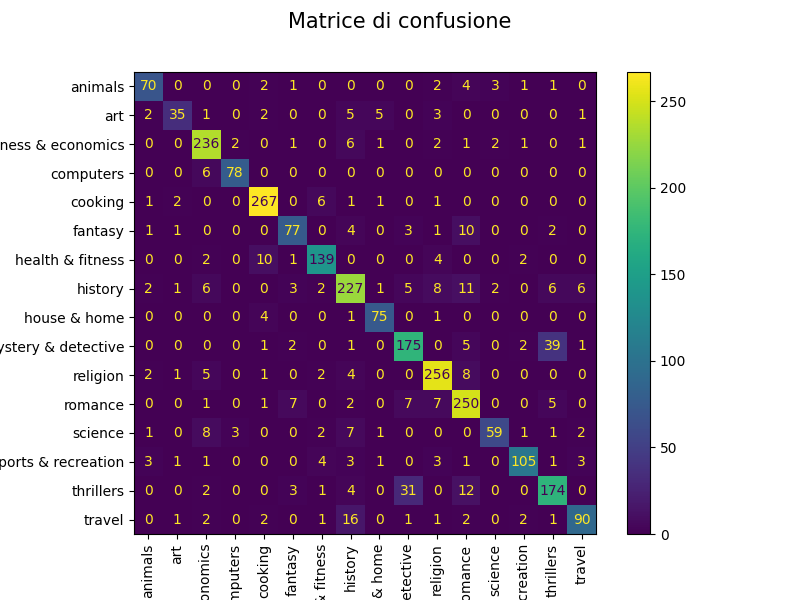
\includegraphics[width=0.95\textwidth]{pics/LinearSVC_confusion_matrix.png}

        
        \begin{justify}
        Si notano risultati decisamente migliori rispetto ai modelli precedenti. Il tempo per l’apprendimento è ancora sufficientemente basso e le predizioni sono state molto più accurate e con meno lacune rispetto le categorie meno frequenti. Dal classification report si nota come la categoria “Art” sia quella con lo score minore (f1-score di 0.74), come ci si poteva aspettare dalla classe con meno esempi nel dataset. In generale, le predizioni effettuate sono abbastanza soddisfacenti. Grazie alla matrice di confusione è possibile notare una tendenza, più evidente rispetto ai modelli precedenti, nel confondere alcune categorie simili. Di fatto un buon numero di libri appartenenti alla categoria “Mistery \& Detective” sono stati confusi come “Thriller” (e viceversa). Osservando i wordcloud delle categorie in questione sono presenti parole chiave comuni (ad esempio: “\textit{murder}”, “\textit{killer}”): risulta dunque evidente la difficoltà nella suddivisione netta delle due tipologie di libri (è una tendenza che ci si aspetta di osservare anche dai successivi classificatori).
    \end{justify}
    \end{enumerate}

    \begin{enumerate}
    
    \subsection{Logistic Regression Classification}
    \begin{justify}
    Il classificatore Logistico, anche detto Regressore Logistico, è una tipologia di classificatore lineare binario. Il suo obiettivo è l’identificazione di una retta (o un piano, nel caso in cui le feature fossero superiori a due) in grado di stimare la probabilità che un esempio faccia parte di una determinata classe piuttosto che di un’altra. Dalla probabilità stimata è poi facile ricondurre la categoria da predire, passando dunque da un problema risolto con un approccio regressivo ad uno di classificazione. Tale algoritmo supporta l’integrazione della tecnica "One-Vs-Rest" per effettuare predizioni multiclasse e risulta essere adatto ad input sotto forma di matrici sparse. Considerando i risultati ottenuti dal classificatore precedente, si è deciso di valutare un ulteriore classificatore lineare, con una tipologia di approccio misto regressione – classificazione.
    Il suo addestramento ha impiegato all’incirca 114.64 secondi, ottenendo un punteggio di accuracy di 0.842. 
    Di seguito ne si riporta il suo classification report e la matrice di confusione delle predizioni:
    \end{justify}

    \centering
    \includegraphics[width=0.80\textwidth]{pics/classificationReport_LogisticRegression.png}
    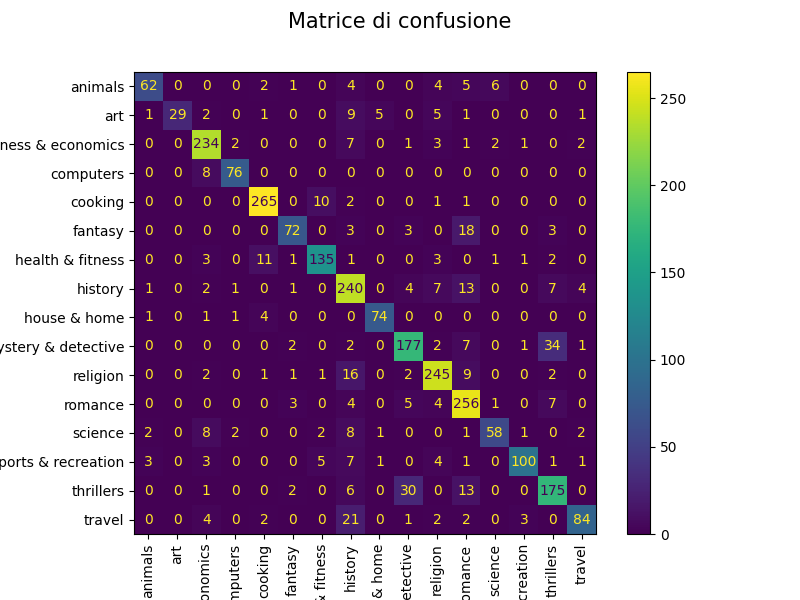
\includegraphics[width=0.95\textwidth]{pics/LogisticRegression_confusion_matrix.png}

    \begin{justify}
    Tra tutti i classificatori provati, questo è il classificatore più lento in fase di addestramento. Com’è noto, gli algoritmi di apprendimento, per problemi di regressione lineare, impiegano molto tempo per apprendere le funzioni lineari che meglio si adattano ai dati, soprattutto se si lavora con dati in larga scala (di numero di righe e numero di feature). Durante i vari test condotti sul regressore logistico è stato molto frequente l'evento in cui l’algoritmo non è stato in grado di convergere ad una soluzione riportando, ovvero un errore. Indipendentemente da ciò, i risultati ottenuti sono di poco al di sotto del classificatore precedente e, in generale, abbastanza soddisfacenti. Si può notare una maggior confusione, rispetto a quanto visto nel Linear Support Vector, verso ulteriori categorie simili, come per esempio “Religion” - “History” e “Fantasy” - “Romance”. Di conseguenza tutti i punteggi f1-score, riportati per le varie categorie, risultano essere più bassi. 
    \end{justify}
    \end{enumerate}

   \begin{enumerate}
    \subsection{Stochastic Gradient Descent Classification}
    \begin{justify}
    Il classificatore Stochastic Gradient Descent non fa parte di una specifica famiglia di modelli di machine learning, ma è una tecnica di ottimizzazione che permette di addestrare un modello di classificazione in maniera efficiente. Secondo la documentazione fornita da Sklearn, a seconda della configurazione degli iperparametri che gli vengono forniti, tale classificatore utilizza specifiche tecniche adottate già da altri modelli con l’obiettivo di ottimizzarle. Tali tecniche si basano su approcci lineari e, visti gli ottimi risultati ottenuti dai precedenti classificatori lineari, sembra ragionevole considerare anche quest’ulteriore classificatore. È un modello adatto per apprendimenti su dati in larga scala, sia in termini di numeri di esempi che di feature per ciascuno di essi. Di conseguenza, dovrebbe risultare ottimo nei problemi di classificazione di testo e, in generale, nel natural language process.
    Il suo addestramento ha impiegato all’incirca 7.23 secondi, ottenendo un punteggio di accuracy di 0.85. Di seguito ne si riporta il suo classification report e la matrice di confusione delle predizioni:
    \end{justify}

    \centering
    \includegraphics[width=0.80\textwidth]{pics/classificationReport_SGDClassifier.png}
    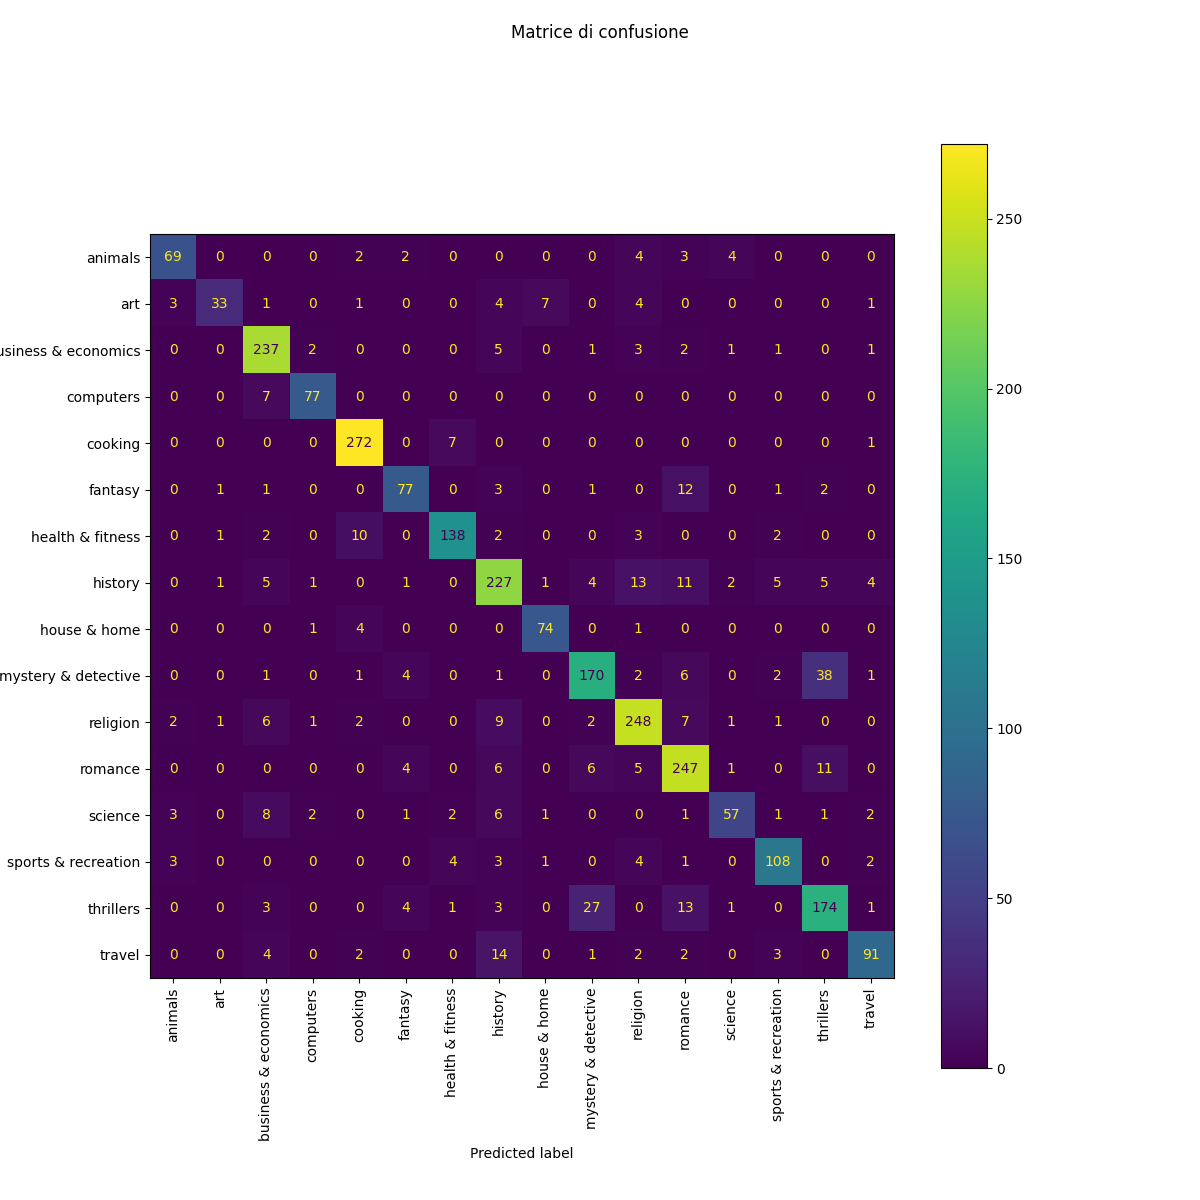
\includegraphics[width=0.95\textwidth]{pics/SGDClassifier_confusion_matrix.png}

    \begin{justify}
    I risultati ottenuti sono molto simili a quelli ricavati dal Linear Support Vector. Tempi di addestramento e punteggi sono del tutto analoghi. Inoltre, durante i vari test condotti sui modelli, si è potuto notare come in effetti nessuno dei due modelli prevalga in assoluto sull’altro.\\
    Per alcuni testi il Linear Support Vector è risultato migliore, per altri, invece, lo è stato SGD. Tale modello rappresenta un’ulteriore prova di come gli approcci lineari risultino ottimi per problemi di classificazione di testo.
    \end{justify}
    \end{enumerate}

    \newpage
    \begin{enumerate}
    \subsection{Valutazioni finali sulla Classificazione}
    \begin{justify}
    Dai risultati ottenuti si evidenzia come i classificatori bayesiani siano del tutto sconsigliabili per problemi di classificazione testuale: seppur abbastanza rapidi nella fase di addestramento, non sembrano adattarsi bene ad uno spazio di esempi con numerose feature e rischiano facilmente di andare in underfitting.\\
    La classificazione tramite approccio regressivo adottata dal regressore lineare sembra essere sufficientemente adeguata a fornire buoni risultati. Tuttavia, la sua scarsa scalabilità a dati di grandi dimensioni lo rende un algoritmo poco efficiente e facilmente impraticabile. Nel nostro caso sono stati utilizzati all’incirca 27000 esempi per l’addestramento. In casi reali, per produrre una soluzione di machine learning sufficientemente addestrata, il numero di esempi dovrebbe essere molto più grande, nonostante il conseguente aumento di complessità per un modello di regressione lineare di arrivare a convergenza.\\
    In conclusione, i modelli lineari (Linear Support Vector e SGD) sono risultati assolutamente i migliori: non solo i punteggi ottenuti sono di gran lunga superiori agli altri tipi di modelli, ma anche i tempi di addestramento, seppur non i più bassi, sono stati sufficientemente contenuti. Inoltre, sono stati in grado di adattarsi in modo ottimale ad un dataset piuttosto sbilanciato e fornire predizioni abbastanza accurate per ogni categoria. La scalabilità verso un quantitativo di dati maggiore, dalle documentazioni riportate dalla libreria Sklearn, l’algoritmo SGD dovrebbe essere progettato e ottimizzato appositamente per lavorare con grandi mole di dati e, per tale motivo, è preferibile rispetto al Linear Support Vector.\\
    Si tenga presente che tutti i modelli hanno avuto chiare difficoltà nel distinguere accuratamente categorie con elementi simili, come per “Mystery \& Detective” – “Thriller” o “Religion” – “History”. Osservando i relativi wordcloud ci si accorge facilmente di parole chiave comuni che potrebbero indurre in confusione. Al fine di rendere più netta la divisione tra le categorie, e dunque ottenere dai modelli risultati migliori, si potrebbe pensare di accorpare categorie con elementi simili (com’è già stato fatto per altre categorie precedentemente presenti nel dataset). Tuttavia, si rischierebbe di avere un set di categorie eccessivamente generiche e, di conseguenza, poco utili nella maggior parte dei contesti pratici.
    \end{justify}
    \end{enumerate}

\newpage
\section{Clustering}
    \begin{justify}
        Nel contesto dell'analisi e dell'organizzazione di un vasto insieme di libri provenienti da un dataset contenente descrizioni e informazioni sugli autori, il clustering, basato sulle regole dell'apprendimento non supervisionato, si presenta, in linea teorica, come un buon approccio alternativo alla classificazione. Questa metodologia ci offre la possibilità di organizzare i libri in gruppi sfruttando contemporaneamente le somiglianze semantiche nelle descrizioni e le ricorrenze degli autori per ogni cluster, così da creare connessioni significative tra opere affini. Conoscendo a priori il numero di categorie differenti presenti nel dataset (16 categorie), si è adottato un approccio che coinvolge algoritmi di clustering in cui il numero di gruppi risultanti sia preimpostato come iperparametro. Questa scelta ci ha permesso di effettuare anche un confronto più accurato con gli algoritmi di classificazione.
        Per ogni modello selezionato sono state calcolate e riportare le seguenti metriche:
        \begin{itemize}
            \item Silhouette score
            \item Tempo necessario per l’addestramento
            \item Top 10 keywords più frequenti contenute nelle descrizioni degli elementi di ogni cluster (vedi immagine sotto)
            \item Top 10 autori più frequenti contenuti negli elementi di ogni cluster (vedi\\ immagine sotto)
        \end{itemize}

        \includegraphics[width=\textwidth]{pics/keywords.PNG}
    \end{justify}
    \begin{enumerate}
    \newpage
    \subsection{Algoritmo K-Means}
    \begin{justify}
        Il K-Means è uno degli algoritmi di clustering più famoso. Il suo obiettivo è quello di raggruppare i dati allo scopo di separare i campioni in K gruppi di uguale varianza, minimizzando un criterio noto come “somma dei quadrati” all'interno del cluster. Possiamo descrivere questo procedimento con i seguenti step:
        \begin{enumerate}[label=\arabic*)]
            \item Scegliere in modo casuale K punti nel dataset come centroidi iniziali;
            \item Generare un partizionamento assegnando ogni campione al centroide più vicino;
            \item Calcolare i nuovi centroidi del cluster considerando la media dei valori del cluster generato al punto 2;
            \item Ripetere i passi 2 e 3 fino a quando i centroidi non cambino.
        \end{enumerate}
        Il suo addestramento ha impiegato all’incirca 17.99 secondi, ottenendo un Silhouette score di 0.006. Di seguito ne si riportano le top 10 keywords più frequenti contenute nelle descrizioni e i top 10 autori più frequenti.
        \end{justify}

        \begin{figure}[H]
        \includegraphics[width=0.90\textwidth]{pics/desc_kmeans.PNG}
        \captionsetup{width=0.90\textwidth, justification=centering}
        \caption{Top 10 keywords più frequenti contenute nelle descrizioni degli elementi di ogni cluster}
        \end{figure}

        \begin{figure}[H]
        \includegraphics[width=0.90\textwidth]{pics/aut_kemans.PNG}
        \caption{Top 10 autori più frequenti contenuti negli elementi di ogni cluster}
        \end{figure}
        
        \begin{justify}
        A questo punto possiamo osservare che, avendo ottenuto un Silhouette score molto vicino allo 0, i cluster ricavati al termine sono sovrapposti. Infatti, anche andando ad analizzare le keywords ottenute, non è molto chiaro per tutti i cluster che genere questi rappresentino. Questi risultati poco incoraggianti ci lasciano come scelta solo quella di analizzare come si comporta un modello di Mini-Batch K-Means in termini di tempo di addestramento (poiché non ci potrà permettere di ottenere risultati migliori) e successivamente affidarci all’abilità di gestire strutture complesse e non lineari nei dati dello Spectral Clustering.
    \end{justify}
    \end{enumerate}

    \begin{enumerate}
    \subsection{Algoritmo MiniBatchKMeans}
    \begin{justify}
    Il Mini-Batch K-Means è una variante dell'algoritmo K-Means standard che utilizza minibatch di campioni, ovvero sottoinsiemi di dati di input campionati casualmente in ogni iterazione di training per aggiornare i centroidi, invece di utilizzare l'intero set di dati. Questo approccio rende Mini-Batch K-Means più efficiente dal punto di vista computazionale permettendo di lavorare su dataset più grandi rispetto al K-Means tradizionale. A differenza di altri algoritmi che riducono il tempo di convergenza, il Mini-Batch K-Means produce risultati che generalmente sono solo leggermente peggiori rispetto all’algoritmo standard. 
    Possiamo descrivere questo algoritmo con i seguenti step:

    \begin{enumerate}[label=\arabic*)]
        \item Scegliere in modo casuale K punti nel dataset come centroidi iniziali;
        \item Ad ogni iterazione, selezionare casualmente un minibatch di dimensione prefissata dal dataset;
        \item Generare un partizionamento assegnando ogni campione del minibatch al centroide più vicino; 
        \item Aggiornare i centroidi usando la media dei punti nel minibatch corrente;
        \item Ripetere i passi da 2 a 4 fino a quando i centroidi non cambiano.
    \end{enumerate}
    Il suo addestramento ha impiegato all’incirca 3.17 secondi, ottenendo un Silhouette score di 0.005. Di seguito ne si riportano le top 10 keywords più frequenti contenute nelle descrizioni e i top 10 autori più frequenti.
    \end{justify}
    \hfill

    \begin{figure}[H]
    \includegraphics[width=0.90\textwidth]{pics/desc_minik.PNG}
    \captionsetup{width=0.90\textwidth, justification=centering}
    \caption{Top 10 keywords più frequenti contenute nelle descrizioni degli elementi di ogni cluster}
    \end{figure}

    \begin{figure}[H]
    \includegraphics[width=0.90\textwidth]{pics/aut_minik.PNG}
    \captionsetup{width=0.90\textwidth, justification=centering}
    \caption{Top 10 autori più frequenti contenuti negli elementi di ogni cluster}
    \end{figure}

    \newpagw
    \begin{justify}
    È possibile notare come questo modello sia nettamente più rapido nell’addestramento rispetto alla versione standard del K-Means (quasi 15 secondi di differenza) ma, come già previsto dalla teoria, il Silhouette score non si abbassa drasticamente.
    \end{justify}
    \begin{justify}
    Il fine dell’implementazione di questo algoritmo è più sperimentale che di utilità. È da considerare che in una possibile futura analisi su un dataset, con le stesse features ma con molti più dati, l’algoritmo Mini-Batch K-Means potrebbe quasi del tutto sostituire K-Means e, talvolta, essere preferibile ad esso.
    \end{justify}
    \end{enumerate}

    \begin{enumerate}
    \subsection{Algoritmo SpectralClustering}
    \begin{justify}
    Lo Spectral Clustering è un algoritmo di clustering che si basa sulla teoria spettrale, ovvero una branca matematica legata allo studio delle proprietà degli spettri degli operatori lineari. Quest'approccio offre un modo potente per affrontare strutture complesse e non lineari nei dati, le quali non possono essere gestite adeguatamente da metodi più tradizionali come K-Means. 
    Il processo di funzionamento può essere suddiviso in diverse fasi:
    \begin{enumerate}[label=\arabic*)]
        \item Utilizzando la similarità tra i punti del dataset (calcolata ad esempio utilizzando la distanza euclidea tra i punti), viene costruito un grafo;
        \item Sfruttando la teoria spettrale, il grafo viene trasformato in uno spazio di dimensioni inferiori attraverso la procedura degli autovettori e degli autovalori;
        \item Una volta ottenuto lo spazio trasformato, viene applicato un algoritmo di clustering, come ad esempio K-Means, per raggruppare i punti in cluster;
        \item I risultati dell'algoritmo di clustering vengono utilizzati per assegnare ciascun punto del dataset a un cluster specifico. La coerenza e la separazione dei cluster dipendono dalla capacità della trasformazione spettrale di rivelare pattern significativi nei dati.
    \end{enumerate}
    Il suo addestramento ha impiegato all’incirca 273.08 secondi, ottenendo un Silhouette score di 0.005. Di seguito ne si riportano le top 10 keywords più frequenti contenute nelle descrizioni e i top 10 autori più frequenti.
    \end{justify}

    \hfill

    \begin{figure}[H]
    \includegraphics[width=0.90\textwidth]{pics/desc_spect.PNG}
    \captionsetup{width=0.90\textwidth, justification=centering}
    \caption{Top 10 keywords più frequenti contenute nelle descrizioni degli elementi di ogni cluster}
    \end{figure}


    \begin{figure}[H]
    \includegraphics[width=0.90\textwidth]{pics/aut_spect.PNG}
    \captionsetup{width=0.90\textwidth, justification=centering}
    \caption{Top 10 autori più frequenti contenuti negli elementi di ogni cluster}
    \end{figure}
    
    \begin{justify}
    Tra tutti gli algoritmi di clustering provati, questo è stato decisamente il più lento, anche con un margine piuttosto evidente. C’era da aspettarselo poiché, oltre che eseguire il K-Means, lo Spectral Clustering richiede ulteriori operazioni preliminari di costruzione di un grafo e trasformazione di esso in uno spazio di dimensioni inferiori. Nonostante il tempo molto disteso per l’addestramento, il Silhouette score ottenuto risulta essere addirittura peggiore di quello ricavato dal K-Means (seppur di poco). Questa valutazione ci permette di capire che l’algoritmo non è stato in grado di rivelare dei pattern significativi nei dati, difficoltà, evidentemente, introdotta dai vari problemi previsti nella gestione del linguaggio naturale.
    \end{justify}
    \end{enumerate}


\newpage
    \begin{enumerate}
    \subsection{Valutazioni finali sul clustering}
    \begin{justify}
        Dallo studio condotto sui vari modelli di clustering si nota come per ognuno di essi i risultati ottenuti non li rendono effettivamente utilizzabili nella pratica. La media dei Silhouette score ottenuti si aggira intorno allo zero e le keywords estratte dalle singole analisi non sono funzionali al riconoscimento della categoria di appartenenza del libro. 
        Nonostante ciò, l’algoritmo che ha portato a risultati migliori, seppur di poco, è stato il K-Means, mentre il più veloce nell’addestramento è stato il Mini-Batch K-Means, il che lo rende anche il più propenso a essere adattato a dataset con un numero molto maggiore di dati.
        Lo Spectral Clustering, invece, non ci ha permesso di giungere a risultati di qualità superiore a causa della rappresentazione stessa dei dati e perchè si tratta di una tecnica tipicamente non utilizzata per dati testuali, ma per dati numerici o geometrici, come quelli provenienti da immagini.
    \end{justify}
    \end{enumerate}


\section{Implementazione script per l'addestramento}
    \begin{justify}
        Com’è già stato specificato precedentemente, al fine di poter addestrare un modello di machine learnig su dati testuali è stato necessario far ricorso a conteggi in frequenze per convertire le parole in sequenze di valori numerici utilizzabili da algoritmi di apprendimento. Per far ciò è stato necessario ricorrere alla classe ‘TfidfVectorizer’, la quale è autonomamente in grado di estrarre i token costituenti i periodi testuali, contarli e normalizzare i conteggi secondo la tecnica tf-idf (term frequency–inverse document frequency). L’output fornito  da tale processo è una matrice sparsa di valori numerici costituita da tante colonne quante sono le differenti parole identificate e tante righe quanti sono gli esempi. Per le descrizioni si è deciso di considerare unicamente token costituiti da parole singole, mentre, per gli autori, si è pensato potesse tornare utile considerare anche token costituiti da due parole (quelle che dovrebbero rappresentare nome e cognome dell’autore).
        \end{justify}
        \hfill
        \includegraphics[width=\textwidth]{pics/tfidtransformer.png}

        \newpage
        \begin{justify}
        Successivamente, lo script costruisce una pipeline contenente i “vettorizzatori” (istanze di TfidfVectorizer’) per le descrizioni e per gli autori e il modello il cui nome viene specificato da uno dei parametri in input.
        \end{justify}

        \begin{figure}[H]
        \includegraphics[width=1\textwidth]{pics/pipeline.png}
        \caption{Pipeline dei classificatori}
        \end{figure}

        \begin{figure}[H]
        \includegraphics[width=1\textwidth]{pics/pipeline2.png}
        \caption{Pipeline dei cluster}
        \end{figure}
        
        \begin{justify}
        In seguito, si passa all’addestramento del modello. Se specificato da uno dei parametri in input, si effettua una ricerca dei migliori parametri di configurazione per il modello (vedere paragrafo ~\ref{ott}), portando ad un addestramento molto più lungo, altrimenti si addestra il modello con una configurazione di default. Infine, se specificato, il modello viene serializzato e memorizzato in un file binario per poter essere, successivamente, recuperato e utilizzato per effettuare predizioni.

        \begin{figure}[H]
        \centering
        \includegraphics[width=1\textwidth]{pics/addestramento.png}
        \includegraphics[width=1\textwidth]{pics/addestramento2.png}
        \end{figure}
        
        \end{justify}

\section{Ottimizzazione modelli}\label{ott}
    \begin{justify}
        Com’è noto, ogni tipo di modello, che sia di classificazione o clustering, possiede una serie di parametri. Questi parametri sono noti come iperparametri e, anche se opportunamente configurati, permettono di addestrare il modello in maniera ottimale e di adattarsi meglio ai dati a disposizione. Ogni modello possiede parametri specifici e la regolazione di essi risulta particolarmente complessa e richiederebbe conoscenze specifiche sul funzionamento dell’algoritmo di addestramento di cui fa uso. Anche assumendo di essere a conoscenza del funzionamento di ciascun algoritmo, risulta comunque complesso e dispendioso dal punto di vista temporale determinare “a mano” i valori per ciascuno dei parametri a disposizione.
        \end{justify}
    \newpage
        \begin{justify}
        Per tale motivo, tipicamente si sceglie di addestrare e valutare lo stesso modello, sugli stessi dati, ma con differenti configurazioni dei parametri, determinando poi quale di queste ha conseguito il risultato migliore. 
        La libreria Sklearn mette a disposizione degli strumenti per automatizzare tale processo: GridSearchCV e RandomizedSearchCV. Entrambe le classi operano nello stesso modo: si indica il modello che si intende addestrare e si specifica una lista dei parametri interessati al “tuning” e dei possibili valori da assegnargli e automaticamente essi addestreranno e valuteranno il modello indicato con differenti permutazioni dei valori specificati per i vari parametri. Nello specifico, ciascun modello viene valutato con un approccio Cross – Validation, per aumentare l’affidabilità della valutazione stessa. La differenza sostanziale tra GridSearch e RandomizedSearch è che il primo addestra e valuta tutti i modelli con tutte le possibili permutazioni di configurazioni specificate mentre il secondo valuta casualmente soltanto un numero predefinito di queste. Ovviamente il primo approccio è esaustivo e permette di identificare con certezza il miglior modello possibile, a discapito di un’enorme quantità di tempo necessaria per la ricerca. Il secondo, invece, è una ricerca meno esaustiva che punta sulla “fortuna della casualità”, ma permette di ottenere dei risultati mediamente migliori di una configurazione dei parametri di default e in tempi molto più brevi.
        Ai fini del nostro progetto, e per le risorse limitate a noi a disposizione, abbiamo comunque deciso di provare ad ottimizzare i nostri modelli ma tramite l’ausilio della RandomizedSearch. C’è da specificare che l’identificazione del miglior modello deve essere fatta sulla base di un punteggio che permetta di determinare quando un modello è migliore di un altro. Nello specifico, per i modelli di classificazione ci si è basati sull’Accuracy, mentre per i modelli di clustering si è usato il Silhouette score. Si tenga conto che un approccio di valutazione Cross Validation, per modelli di clustering, non ha molta utilità e per tale motivo questo tipo di valutazione è stata usata solo per modelli di classificazione.
        \end{justify}

        \begin{figure}[H]
        \includegraphics[width=0.70\textwidth]{pics/parametri.png}
        \captionsetup{width=0.70\textwidth, justification=centering}
        \caption{Parametri e valori considerati per l’ottimizzazione di alcuni dei modelli di classificazione}
        \end{figure}

        \begin{figure}[H]
        \includegraphics[width=0.70\textwidth]{pics/parametri2.png}
        \captionsetup{width=0.70\textwidth, justification=centering}
        \caption{Parametri e valori considerati per l’ottimizzazione di alcuni dei modelli di clustering}
        \end{figure}
        
        \begin{justify}
        Si riportano i risultati ottenuti dall’ottimizzazione di un modello di classificazione e uno di clustering.
        Per la classificazione, si è tentata l’ottimizzazione del modello Linear Support Vector: la ricerca ha impiegato all’incirca 1130.68 secondi ottenendo un punteggio di accuracy di 0.855. Di seguito ne si riporta il suo classification report e la matrice di confusione delle predizioni:
        \end{justify}

        \centering
        \includegraphics[width=0.80\linewidth]{pics/classificationReport_LinearSVC_best.png}
        
        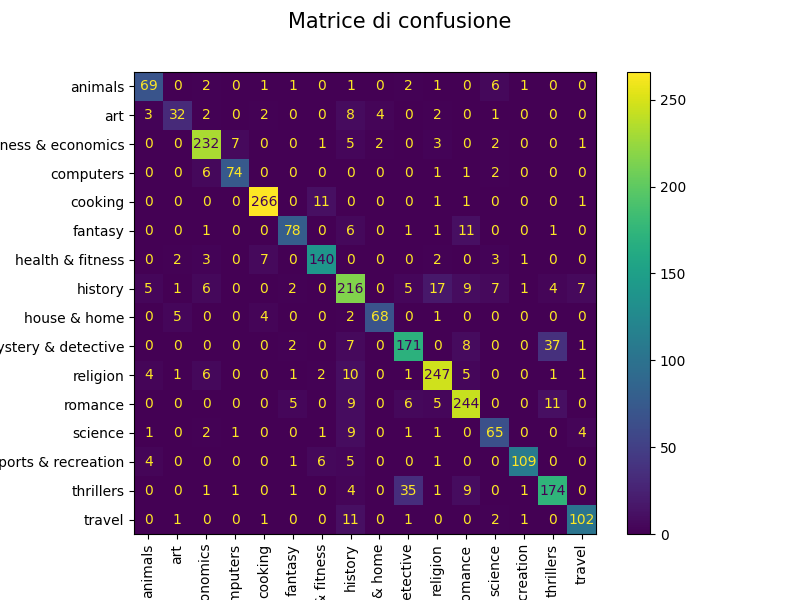
\includegraphics[width=0.80\linewidth]{pics/LinearSVC_best_confusion_matrix.png}
        
        \begin{justify}
        Per il clustering, si è tentata l’ottimizzazione del modello K-Means: la ricerca ha impiegato all’incirca 236.51 secondi ottenendo un Silhouette score di 0.011.
        \end{justify}

        \begin{figure}[H]
        \includegraphics[width=0.70\linewidth]{pics/key_des_best.PNG}
        \captionsetup{width=0.70\textwidth, justification=centering}
        \caption{Top 10 keywords più frequenti contenute nelle descrizioni degli elementi di ogni cluster}
        \end{figure}

        \begin{figure}[H]
        \includegraphics[width=0.70\linewidth]{pics/key_aut_best.PNG}
        \captionsetup{width=0.70\textwidth, justification=centering}
        \caption{Top 10 autori più frequenti contenuti negli elementi di ogni cluster}
        \end{figure}

        \begin{justify}
        Confrontando i risultati ottenuti dai modelli “ottimizzati” con le rispettive versioni “non ottimizzate” si può notare come, in effetti, essi non siano tanto migliori e, anzi, hanno raggiunto punteggi simili. L'esito non stupisce considerando che: 
        \begin{itemize}
            \item La ricerca RandomizedSearch è un processo casuale che non garantisce l’ottimalità;
            \item Non avendo conoscenze dettagliate sul funzionamento tecnico degli algoritmi in questione, probabilmente la lista dei parametri indicati e i rispettivi valori specificati potrebbero non essere adatti, o comunque, potrebbero essere specificati valori maggiormente sensati;
            \item Non è da escludere la possibilità per cui le configurazioni predefinite, usate per le versioni “non ottimizzate” dei modelli, siano già efficaci a ottenere il miglior risultato possibile utilizzando i dati disponibili.
        \end{itemize}
    \end{justify}

    \section{Conclusioni}
    \begin{justify}
        Dopo aver condotto addestramenti approfonditi su ciascun modello di classificazione e clustering, accompagnati da dettagliati report analitici e successiva ottimizzazione del modello più promettente, emergono come rappresentativi della rispettiva categoria il Linear Regression e l'algoritmo K-Means.
        Nel confronto tra i due modelli, si evidenzia chiaramente la superiorità del Linear Regression rispetto alle prestazioni più limitate del K-Means. 
        Mentre i cluster identificati da K-Means risultano poco significativi e poco coesi rendendo quest'algoritmo inutilizzabile per la nostra applicazione pratica, le analisi condotte sul Linear Regression indicano che questo modello è capace, nella maggior parte dei casi, di assegnare con precisione la categoria di un libro. Un vantaggio notevole è dato anche dal tempo di addestramento, significativamente inferiore rispetto a quello della sua controparte di apprendimento non supervisionato.
        \end{justify}

        \begin{justify}
        Questi risultati sottolineano chiaramente che, nel nostro contesto di categorizzazione dei libri, la metodologia più adatta è la classificazione. Quest’approccio, infatti, offre modelli specificamente progettati per lavorare su dati testuali garantendo una maggiore precisione e pertinenza rispetto al clustering, in cui si utilizzano approcci più generici e meno specifici per la gestione di dati in linguaggio naturale. 
    \end{justify}

    \begin{textblock*}{8cm}(12cm,22cm)
    Mancuso Maria Angela 0612705832\\
    Malfettone Ines 0612705311\\
    Santonicola Federico 0612706449\\
    Sessa Attilio Marco 0612705403
\end{textblock*}
\end{document}
